\documentclass[10pt,a4paper]{article}
\usepackage[margin=2.2cm]{geometry}
\usepackage{fontspec}
\usepackage{xeCJK}
\setCJKmainfont{SimSun}[BoldFont=SimHei]
\setCJKsansfont{SimHei}
\usepackage{amsmath}
\usepackage{graphicx}
\usepackage{booktabs}
\usepackage{array}
\usepackage{caption}
\usepackage{enumitem}
\usepackage[hidelinks]{hyperref}
\setlist{nosep,leftmargin=1.5em}
\linespread{1.25}
\captionsetup{font=small}
\renewcommand{\figurename}{图}
\renewcommand{\tablename}{表}
\renewcommand{\contentsname}{目录}
\newcommand{\dn}{\Delta n_0}

\title{\textbf{长孔径分段馈电薄膜铌酸锂声光相位调制器：仿真进展报告}}
\author{陈鑫磊\quad 上海电力大学}
\date{2026 年 10 月 22 日}

\begin{document}
\maketitle

\noindent\fbox{\parbox{\dimexpr\linewidth-2\fboxsep-2\fboxrule}{\small
\textbf{本稿仅限课题组内部：仿真与方案工作稿，实测待做，无伪造数据，Fiber-Q 未下单，无流片；不得作为公开或可引用结果。}
文中全部器件数字均为 COMSOL 仿真预测，不是实验结果。}}

\section{结论摘要}
\begin{itemize}
  \item 设计：悬空 X 切铌酸锂（400 nm），Shao 取向（声沿晶体 Z 传播，TE 光沿晶体 Y，主要利用 $r_{33}$ 与光弹效应），
        400 nm 高脊波导嵌在叉指中间，谐振约 3.2--3.3 GHz，波长 1550 nm。
  \item 单位长度效率：有限长模型给出 $P_\pi L = 2.4$--$2.9\times10^{-6}$ W·m，与同一流程算出的 Shao 型结构（$2.36\times10^{-6}$）相当（1.0--1.2 倍）。
        单位长度效率\textbf{没有}超过 Shao 型；优势来自下一条。
  \item 长孔径与馈电：孔径拉到毫米级，叉指按段（段长 $\ge 25\ \mu$m）串联/并联组合，总阻抗配到 33--72 $\Omega$，计入分布 RC 电极电阻。
        $L = 1$ mm 时 $\pi$ 相移所需信号源功率 2.5--3.1 mW（等效 $V_\pi \approx 0.5$ V，50 $\Omega$）。
  \item 三维校核（第~\ref{sec:3d} 节）：计入汇流条、指端和段间隙后，单个主模分裂成一串相邻模式，
        $P_\pi L$ 变为 $4.8$--$6.4\times10^{-6}$ W·m（二维的 2.0--2.6 倍）；段长 25 与 50 µm 结果相近。
        $L = 1$ mm 信号源功率 \textbf{4.8--6.5 mW}，此时 20--40 段全部并联即接近 50 $\Omega$。
  \item 模型偏差：同流程对 Shao 已发表结构的 $\dn$ 偏高 1.3--2.3 倍，功率需乘 1.7--5.3。
        与三维结果相乘后 $L = 1$ mm 约 \textbf{8--34 mW}（两者可能部分重复，合理估计为十几 mW 量级）。
        作为参照，Shao 等实测器件（0.1 mm）需 4.6 V（约 210 mW）。
  \item 查新（初步网页检索）：未见“薄膜铌酸锂长孔径 + 分段串并联配 50 $\Omega$”的报道；
        最接近的是 Freedman 等 2025（AlN--SiN$_x$，2 mm，单段电极 149 $\Omega$，未匹配）。
\end{itemize}

\section{结构与方法}
\begin{figure}[h]
  \centering
  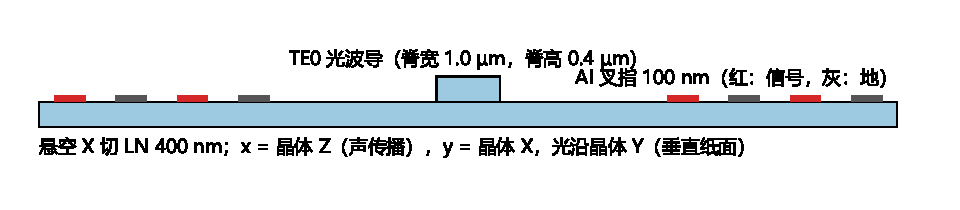
\includegraphics[width=0.95\linewidth]{fig_xsec.pdf}
  \caption{二维截面示意（NP = 7，中间 3 个周期去掉叉指放波导；比例近似）。光沿垂直纸面方向传播，孔径长度 $L$ 也沿这个方向。}
\end{figure}

\begin{itemize}
  \item 二维截面模型（COMSOL 6.3）：压电 + 固体力学本征/频域，光学模式分析；单声子折射率调制 $\dn$ 包括界面移动、光弹、电光三项。
  \item 叉指周期 1.9277 µm（铝指宽 $0.25p$，厚 100 nm），损耗因子 $\eta_s = 5\times10^{-4}$，由此 $Q\approx2000$（假设值，功率 $\propto 1/Q$）。
  \item 两种边界：周期超胞（NP 个周期重复），和有限长（两端自由，对应刻槽释放的悬空膜，与 Shao 器件相同）。
  \item 匹配、电极无损时 $P_\pi L = \hbar\omega^2\lambda^2/(4QL_a\dn^2)$（$L_a = 100\ \mu$m），已与频域驱动结果互相验证。
  \item 电极：每段按分布 RC 传输线计算（$Z_{\rm seg} = (r/\gamma)\coth(\gamma l/2) + rl/2$），$K$ 段 $s$ 串 $\times$ $q$ 并，
        50 $\Omega$ 信号源，计入失配，给出信号源可用功率；汇流条与段间隔离按理想处理。
  \item 校准：同一流程复现 Shao 2019 结构，模式类型一致，$\dn$ 比文献表 S1 高 1.3--2.3 倍（几何从图中估计，有几十 \% 的不确定度）。
\end{itemize}

\section{主要结果}
\subsection{取向与脊高}
把晶体取向转到 Shao 取向后，同流程 $P_\pi L$ 从 $4.9\times10^{-3}$ 降到 $2.2\times10^{-5}$ W·m（约 220 倍），电光项成为主导。
脊高是第二个杠杆（表~\ref{tab:ridge}、图~\ref{fig:ridge}）：100 → 400 nm，$P_\pi L$ 再降 7 倍，TE0 损耗也大幅降低。

\begin{minipage}[c]{0.52\linewidth}
\centering\small
\captionof{table}{脊高扫描（周期超胞 NP = 7，周期 1.9389 µm）}\label{tab:ridge}
\begin{tabular}{cccc}
\toprule
脊高 & $f$ (GHz) & $\dn$ ($10^{-12}$) & $P_\pi L$ (W·m) \\
\midrule
100 nm & 3.358 & 87.6 & $1.78\times10^{-5}$ \\
200 nm & 3.353 & 130.4 & $8.0\times10^{-6}$ \\
300 nm & 3.343 & 169.0 & $4.7\times10^{-6}$ \\
400 nm & 3.311 & 231.4 & $2.48\times10^{-6}$ \\
\midrule
Shao 型 & 3.162 & 219.7 & $2.36\times10^{-6}$ \\
\bottomrule
\end{tabular}
\end{minipage}\hfill
\begin{minipage}[c]{0.44\linewidth}
\centering
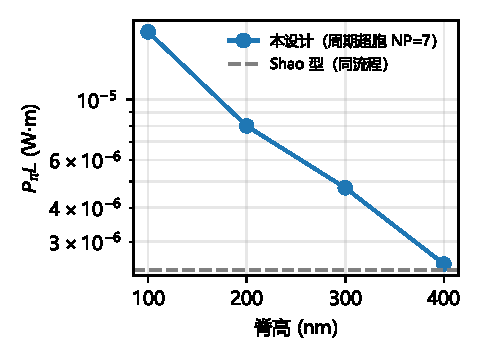
\includegraphics[width=\linewidth]{fig_ridge.pdf}
\captionof{figure}{$P_\pi L$ 随脊高变化。}\label{fig:ridge}
\end{minipage}

\subsection{超胞收敛与有限长校核}
400 nm 脊下，周期超胞结果随 NP 来回波动约 1.8 倍（NP = 9 与一个剪切主导模混合并分裂成两峰）。
改用两端自由的有限长模型后，三种 NP 的结果收敛到 1.2 倍以内（表~\ref{tab:fin}）。
有限长结构的谐振频率比超胞低 2--3.5\%，需把周期缩到约 1.86--1.89 µm 才能回到 3.33 GHz（按 $f\propto1/p$ 估算，待验证）；
$P_\pi L$ 对周期的小幅调整不敏感（周期 1.9389 → 1.9277 µm 时 2.48 → 2.46 $\times10^{-6}$）。

\begin{table}[h]
\centering\small
\caption{脊高 400 nm、周期 1.9277 µm：周期超胞与有限长对比。最后一列为 $L = 1$ mm 按段配 50 $\Omega$ 后的信号源功率。}\label{tab:fin}
\begin{tabular}{llcccccc}
\toprule
边界 & NP & $f$ (GHz) & $\dn$ ($10^{-12}$) & Re$Y$ (S/m) & $P_\pi L$ (W·m) & 分组 & $P_\pi$ @1 mm \\
\midrule
周期 & 7  & 3.326 & 233.7 & 567  & $2.46\times10^{-6}$ & 4 串 × 8 并，30 $\Omega$ & 2.76 mW \\
周期 & 9  & 3.321 & 168.7 & 725  & $4.54\times10^{-6}$ & 8 串 × 4 并，92 $\Omega$ & 5.20 mW \\
周期 & 11 & 3.310 & 201.0 & 1523 & $3.28\times10^{-6}$ & 8 串 × 4 并，45 $\Omega$ & 3.53 mW \\
\midrule
有限长 & 7  & 3.211 & 226.7 & 90  & $2.43\times10^{-6}$ & 2 串 × 16 并，47 $\Omega$ & 2.46 mW \\
有限长 & 9  & 3.241 & 211.0 & 223 & $2.84\times10^{-6}$ & 4 串 × 8 并，72 $\Omega$ & 2.98 mW \\
有限长 & 11 & 3.263 & 210.7 & 509 & $2.90\times10^{-6}$ & 4 串 × 8 并，33 $\Omega$ & 3.11 mW \\
\bottomrule
\end{tabular}
\end{table}

\subsection{分段串并联馈电}
\begin{minipage}[c]{0.50\linewidth}
不分段时，长孔径的阻抗只有几欧，铝指电阻也随长度增大，匹配和电阻损耗使长器件失去意义（$L = 1$ mm 时 0.7--1.4 $\Omega$，需要 35--70:1 变换比）。
按段串并联后（段长 $\ge 25$ µm），各长度下总阻抗都在 27--111 $\Omega$，失配损耗 $< 15\%$。
信号源功率近似按 $1/L$ 下降（图~\ref{fig:power}）：
有限长模型 $L$ = 0.1 / 1 / 2 mm 时分别为 29--31 / 2.5--3.1 / 1.3--1.5 mW。
\end{minipage}\hfill
\begin{minipage}[c]{0.46\linewidth}
\centering
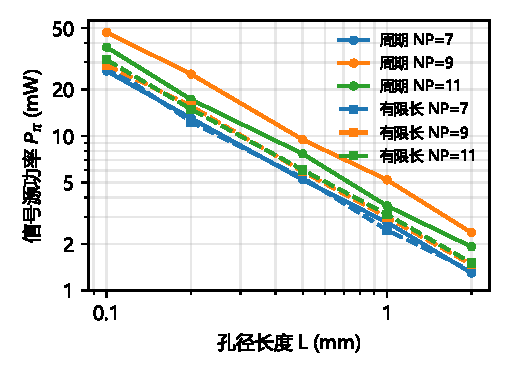
\includegraphics[width=\linewidth]{fig_power.pdf}
\captionof{figure}{按段配 50 $\Omega$ 后 $\pi$ 相移所需信号源功率（二维有限长，未计模型偏高）。}\label{fig:power}
\end{minipage}

\subsection{三维分段校核}\label{sec:3d}
二维截面沿波导方向拉伸成一个分段单元：段间隙 0.5 µm、汇流条 2 µm、指端间隙 0.5 µm、中间为叉指重叠区，
沿波导方向周期边界，两侧自由。光模取自二维模式解，按网格插值读入。
不带汇流条的三维切片与二维有限长相差约 1.5\%（$P_\pi L$ 2.47 对 $2.43\times10^{-6}$），验证了取向、光模映射与网格。

\begin{figure}[h]
  \centering
  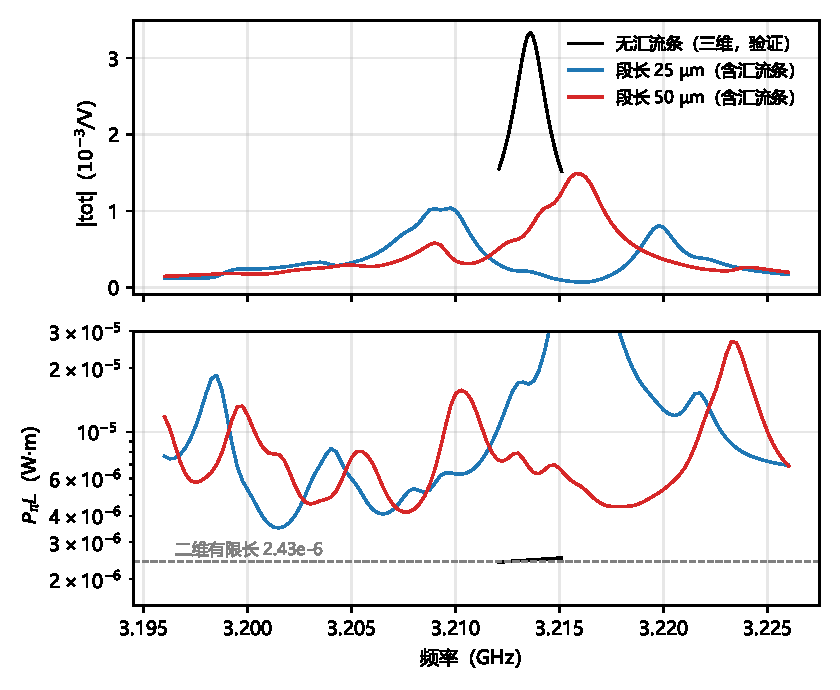
\includegraphics[width=0.54\linewidth]{fig_3d.pdf}
  \caption{三维分段单元的频域驱动响应（截面网格 150/200 nm，沿波导 600/900 nm）。
  上：调制系数 $|{\rm tot}|$；下：$P_\pi L$（匹配、电极无损）。虚线为二维有限长结果。}\label{fig:3d}
\end{figure}

\begin{table}[h]
\centering\small
\caption{三维分段结果（脊 400 nm，NP = 7）。B25 三行为不同网格；最后一列为 $L = 1$ mm 按段配 50 $\Omega$ 的信号源功率。}\label{tab:3d}
\begin{tabular}{lccccccc}
\toprule
段长 / 网格 & $f$ (GHz) & $|{\rm tot}|$ (/V) & Re$Y$ (S/m) & 驱动 $Q$ & $P_\pi L$ 主峰 & 主峰内最小 & $P_\pi$ @1 mm \\
\midrule
无汇流条 & 3.214 & $3.33\times10^{-3}$ & 91 & 2060 & $2.47\times10^{-6}$ & — & — \\
25 µm，150/600 & 3.210 & $1.04\times10^{-3}$ & 23 & 1094 & $6.38\times10^{-6}$ & $4.12\times10^{-6}$ & 6.50 mW \\
25 µm，150/900 & 3.209 & $1.23\times10^{-3}$ & 24 & 1889 & $4.76\times10^{-6}$ & $3.74\times10^{-6}$ & 6.19 mW \\
25 µm，200/400 & 3.210 & $1.33\times10^{-3}$ & 30 & 2210 & $5.03\times10^{-6}$ & $4.55\times10^{-6}$ & 5.61 mW \\
50 µm，200/900 & 3.216 & $1.49\times10^{-3}$ & 42 & 1220 & $5.70\times10^{-6}$ & $4.43\times10^{-6}$ & 4.79 mW \\
\bottomrule
\end{tabular}
\end{table}

\begin{itemize}
  \item 汇流条与指端使原来的单个主模分裂为 3.20--3.22 GHz 内一串间距 0.3--1 MHz 的模式，$\dn$ 分散到几个模上（单模最大 113--152，无汇流条时 225）。
        损失 2.0--2.6 倍，明显大于只按叉指覆盖比例（76\%/88\%）估计的 1.1--1.3 倍。
  \item 段长 25 → 50 µm 无明显改善。主峰高度与宽度随网格变化（几个模式只差几十 kHz），只能给区间；实际器件对加工偏差同样敏感。
  \item 三维中每段的动生电导降低 2--4 倍，段阻抗升高：$L = 1$ mm 时全部并联已接近 50 $\Omega$，只有 $L \ge 2$ mm 才用到串联。
        分段在三维下的主要作用是把指长限制在几十 µm 并均匀馈电，新意表述需相应调整。
\end{itemize}

\section{与已发表工作的对比（初步查新）}
\begin{table}[h]
\centering\small
\caption{相关工作。前五行为文献实测值；最后一行是本工作仿真预测，不能与实测直接比较。}
\begin{tabular}{p{4.3cm}p{3.1cm}p{1.1cm}p{5.9cm}}
\toprule
工作 & 平台 & 长度 & 报道指标 \\
\midrule
Shao 等，Optica 2019 & 悬空 TFLN，1550 nm & 100 µm & 3.33 GHz，$V_\pi = 4.6$ V（MZI） \\
Hassanien 等，Photon.\ Res.\ 2021 & 悬空 TFLN & 45 µm & 1.9 GHz，0.0166 rad/$\sqrt{\rm mW}$，带宽 140 MHz \\
Wan 等，LSA 2022 & TFLN--硫系玻璃，非悬空 & — & 推挽 MZI，$V_\pi L = 0.03$ V·cm \\
Freedman 等，Nat.\ Commun.\ 2025 & AlN--SiN$_x$，730 nm & 2 mm & 2.31 GHz，$V_\pi = 1.32$ V，单段电极 149 $\Omega$ \\
Ni 等，arXiv 2026 & TFLN，非悬空 & 400 µm & 0.842 GHz，$V_\pi L = 1.004$ V·cm \\
\midrule
本工作（仿真） & 悬空 TFLN，1550 nm & 1 mm & 3.2 GHz，三维 $P_\pi$ = 4.8--6.5 mW（修正后 8--34 mW），分段配 50 $\Omega$ \\
\bottomrule
\end{tabular}
\end{table}

\begin{itemize}
  \item “毫米级长孔径”本身不新（Freedman 2025）；可主张的新意是：薄膜铌酸锂上的毫米级孔径，加上计入分布电阻的分段串并联馈电，使阻抗可配到 50 $\Omega$。
  \item 分段电极配 50 $\Omega$ 见于薄膜铌酸锂电光调制器（Optics Express 2025），声光方向未检索到；中文专利（CN114859579A 等）亦未涉及。
  \item 本次只做了网页检索（英文 6 次、中文 1 次），未查 Web of Science、CNKI 全文和专利库全文，不能代替正式查新。
\end{itemize}

\section{风险与下一步}
\begin{enumerate}
  \item \textbf{模型偏高}：对 Shao 结构 $\dn$ 偏高 1.3--2.3 倍；$Q\approx2000$ 是假设值，铝无声学阻尼。功率可能再高数倍。
  \item \textbf{三维模式分裂}：已做三维校核（第~\ref{sec:3d} 节），汇流条带来 2.0--2.6 倍损失。
        下一步：同流程三维 Shao 型（使对比口径一致）；加宽段间隙、段间声学隔离槽或减窄汇流条，看能否抑制分裂。
  \item \textbf{电极网络}：汇流条电阻、段间隔离、寄生电容未计入；串联段之间的电压均分依赖各段谐振一致，对工艺偏差敏感。
  \item \textbf{频率回调}：有限长结构需把周期调到约 1.86--1.89 µm，并验证。
  \item \textbf{去向}：补齐 2、3 两项及工艺容差后，可尝试 Optics Express / JLT 一档的设计型文章；
        若课题组能流片验证，分量会显著提高。投稿与否须经导师和课题组同意。
\end{enumerate}

\section*{附：文件}
\footnotesize\sloppy
仓库目录 \texttt{dir11/comsol\_ao\_run/step6\_optics/}：模型源码 \texttt{Step6j.java}（\texttt{FN} 前缀为有限长）；
日志 \texttt{step6j\_*.log}；匹配计算 \texttt{post\_step6j\_match.py} → \texttt{step6j\_match.log}；
三维模型 \texttt{Step7.java}，日志 \texttt{step7\_*.log}，匹配 \texttt{post\_step7\_match.py} → \texttt{step7\_match.log}；
详细记录 \texttt{summary\_step6i.md}、\texttt{summary\_step6j.md}、\texttt{summary\_step7.md}；本报告与作图脚本在 \texttt{report/}。

\end{document}
